\documentclass[aspectratio=169,xcolor={dvipsnames}
,hide notes
%,show only notes
%,show notes on second screen=right
]{beamer}
\usetheme[background=light, numbering=fraction]{metropolis}
\usepackage{appendixnumberbeamer}

\usepackage[labelfont=bf,textfont={it}]{caption}
\usepackage{subcaption}
\captionsetup[figure]{justification=centering}
\captionsetup[subfigure]{justification=centering}

%\usepackage{fontspec}
%\setsansfont{Fira Sans Mono}

\usepackage[binary-units]{siunitx}
\sisetup{range-phrase=--, range-units=single}

\usepackage[UKenglish]{babel}
\usepackage{csquotes}

\usepackage{amssymb}

\usepackage{lipsum}
\usepackage[basic]{complexity}
\usepackage[super,negative]{nth}

\usepackage{booktabs}

%bib
\usepackage[maxnames=3,maxbibnames=99,mincrossrefs=5,sortcites
,backend=bibtex
,style=authortitle
]{biblatex}
\addbibresource{papers-off.bib}
\addbibresource{confs-off.bib}
\addbibresource{books-off.bib}
\addbibresource{rfc.bib}
\addbibresource{misc.bib}

%picky abt et al.
\usepackage{xpatch}

\xpatchbibmacro{name:andothers}{%
	\bibstring{andothers}%
}{%
	\bibstring[\emph]{andothers}%
}{}{}

%opening!

\usepackage{cleveref}
\newcommand{\crefrangeconjunction}{--}

\usepackage{fontawesome}

%-------------------------------------%
%-------------------------------------%

\title{Reinforcement Learning in Network Defence/Control (WIP)}
\author{Kyle A. Simpson\\
	\small{\faGithub{} \href{https://github.com/felixmcfelix}{FelixMcFelix} \hspace{0.5em} \faGlobe{} \url{https://mcfelix.me}}}
\institute{University of Glasgow}
\date{\nth{10} April, 2018}

\begin{document}

\maketitle

\section{Reinforcement learning}

\begin{frame}{Introducing: Reinforcement Learning}
	\begin{itemize}
		\item Goal: train an agent to make optimal decisions based on observed state.
		\begin{itemize}
			\item Formally, maximise the \alert{expected discounted reward}\footcite{RL2E}.
		\end{itemize}
	
		\item Underlying theory: systems as (discrete-time) \alert{Markov Decision Processes}---states, actions, rewards and transition probabilities.
		\begin{itemize}
			\item I.e., choosing action $a_t$ from a policy in state $s_t$, $a_t \sim \pi(s_t)$, induces the next state $s_{t+1}$ and an associated reward $r_{t+1}$ stochastically.
			\item Generalises to \alert{value} $Q(s,a)$---how much reward can we \emph{eventually} expect from choosing each action currently available?
		\end{itemize}
	\end{itemize}
\end{frame}

\begin{frame}{Why have RL in networks?}
	Link to recent work in data-driven networking/optimisation?
	
	Link to that one GMM paper w/ RL communication.
\end{frame}

\section{What I'm working on}

\begin{frame}{MARL for DDoS prevention}
	Network Model
	
	Pushback
	
	Group reward functions etc.
\end{frame}

\begin{frame}{The case for finer granularity}
	\begin{columns}
	\begin{column}{0.45\linewidth}
		\begin{itemize}
			\item Reduced service guarantees by nature of \emph{pushback} model.
			\begin{itemize}
				\item \alert{Worse with good-faith TCP congestion avoidance}.
			\end{itemize}
			%This is exacerbated by TCP congestion avoidance---legit hosts will be punished far more severely, bad actors don't care!
			
			\item More granular $\implies$ should focus on flow stats, \alert{not aggregates} like now! %Alongside this higher-granularity view, reformulation to include flow characteristics in the decision-making process.
		\end{itemize}
	\end{column}
	\begin{column}{0.5\linewidth}
		\begin{figure}
			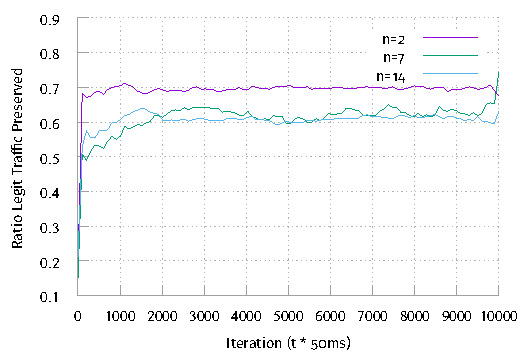
\includegraphics[width=\linewidth]{../plots/online.pdf}
			\caption{Service quality decreases as actions become less granular.}
		\end{figure}
	\end{column}
	\end{columns}
\end{frame}

\section{The adversarial setting}

\begin{frame}{Attacks}
	Poisoning attacks---explain.
	
	Evasion attacks---yes. These are what are often known as `adversarial examples'!
\end{frame}

\begin{frame}{The capabilities of attackers}
	Evasion for \emph{polymorphic blending attacks} on past models are known \NP-Complete. ?? How do they differ from modern perturbations, which are solved by stochastic optimisation?
	
	We have empirically measured bounds on the effectiveness of poisoning attacks wrt.\ what percentage of inbound traffic they can control.
	
	We don't have results for this on e.g., Deep RL in the network.
	
	We also lack results on how/if evasion attacks can transfer for learners focused on non-stationarity/constant learning.
\end{frame}

\begin{frame}[standout]{Conclusion}
	We've looked at...
	\begin{itemize}
		\item A quick introduction to RL, and its \alert{importance to future networks}.
		\item A `direct control' approach to intrusion prevention, and \alert{intended improvements}.
		\item Adversarial work, security, and open questions.
	\end{itemize}
	
	\alert{Questions?}
\end{frame}

\appendix

\begin{frame}[allowframebreaks]{References}
\printbibliography[heading=none]
\end{frame}

\end{document}
